\documentclass[12pt,letterpaper]{article}
\usepackage{graphicx,textcomp}
\usepackage{natbib}
\usepackage{setspace}
\usepackage{fullpage}
\usepackage{color}
\usepackage[reqno]{amsmath}
\usepackage{amsthm}
\usepackage{fancyvrb}
\usepackage{amssymb,enumerate}
\usepackage[all]{xy}
\usepackage{endnotes}
\usepackage{lscape}
\newtheorem{com}{Comment}
\usepackage{float}
\usepackage{hyperref}
\newtheorem{lem} {Lemma}
\newtheorem{prop}{Proposition}
\newtheorem{thm}{Theorem}
\newtheorem{defn}{Definition}
\newtheorem{cor}{Corollary}
\newtheorem{obs}{Observation}
\usepackage[compact]{titlesec}
\usepackage{dcolumn}
\usepackage{tikz}
\usetikzlibrary{arrows}
\usepackage{multirow}
\usepackage{xcolor}
\newcolumntype{.}{D{.}{.}{-1}}
\newcolumntype{d}[1]{D{.}{.}{#1}}
\definecolor{light-gray}{gray}{0.65}
\usepackage{url}
\usepackage{listings}
\usepackage{color}

\definecolor{codegreen}{rgb}{0,0.6,0}
\definecolor{codegray}{rgb}{0.5,0.5,0.5}
\definecolor{codepurple}{rgb}{0.58,0,0.82}
\definecolor{backcolour}{rgb}{0.95,0.95,0.92}

\lstdefinestyle{mystyle}{
	backgroundcolor=\color{backcolour},   
	commentstyle=\color{codegreen},
	keywordstyle=\color{magenta},
	numberstyle=\tiny\color{codegray},
	stringstyle=\color{codepurple},
	basicstyle=\footnotesize,
	breakatwhitespace=false,         
	breaklines=true,                 
	captionpos=b,                    
	keepspaces=true,                 
	numbers=left,                    
	numbersep=5pt,                  
	showspaces=false,                
	showstringspaces=false,
	showtabs=false,                  
	tabsize=2
}
\lstset{style=mystyle}
\newcommand{\Sref}[1]{Section~\ref{#1}}
\newtheorem{hyp}{Hypothesis}

\title{Problem Set 1}
\date{Due: October 1, 2023}
\author{Tolga Bag}

\begin{document}
	\maketitle
	
	\section*{Instructions}
	\begin{itemize}
	\item Please show your work! You may lose points by simply writing in the answer. If the problem requires you to execute commands in \texttt{R}, please include the code you used to get your answers. Please also include the \texttt{.R} file that contains your code. If you are not sure if work needs to be shown for a particular problem, please ask.
\item Your homework should be submitted electronically on GitHub.
\item This problem set is due before 23:59 on Sunday October 1, 2023. No late assignments will be accepted.
\item Total available points for this homework is 80.
	\end{itemize}
	
	\vspace{1cm}
	\section*{Question 1 (40 points): Education}

A school counselor was curious about the average of IQ of the students in her school and took a random sample of 25 students' IQ scores. The following is the data set:\\


\lstinputlisting[language=R, firstline=36, lastline=36]{PS01_TB_23371290.R}  

\vspace{1cm}

\begin{enumerate}
	\item Find a 90\% confidence interval for the average student IQ in the school.\\
	
	\noindent I calculated the mean, variability, standard deviation and standard error. I made them vectors for convenience. \\
	\lstinputlisting[language=R, firstline=41, lastline=45]{PS01_TB_23371290.R}  
	\noindent  I check the distribution of the y. It is normal distribution per Figure 1. I calculate the quantile percentages per the 90\% confidence interval. \\
		\begin{figure}[h!]\centering
		\caption{\footnotesize Distribution of Y}
		\label{fig:plot_1}
		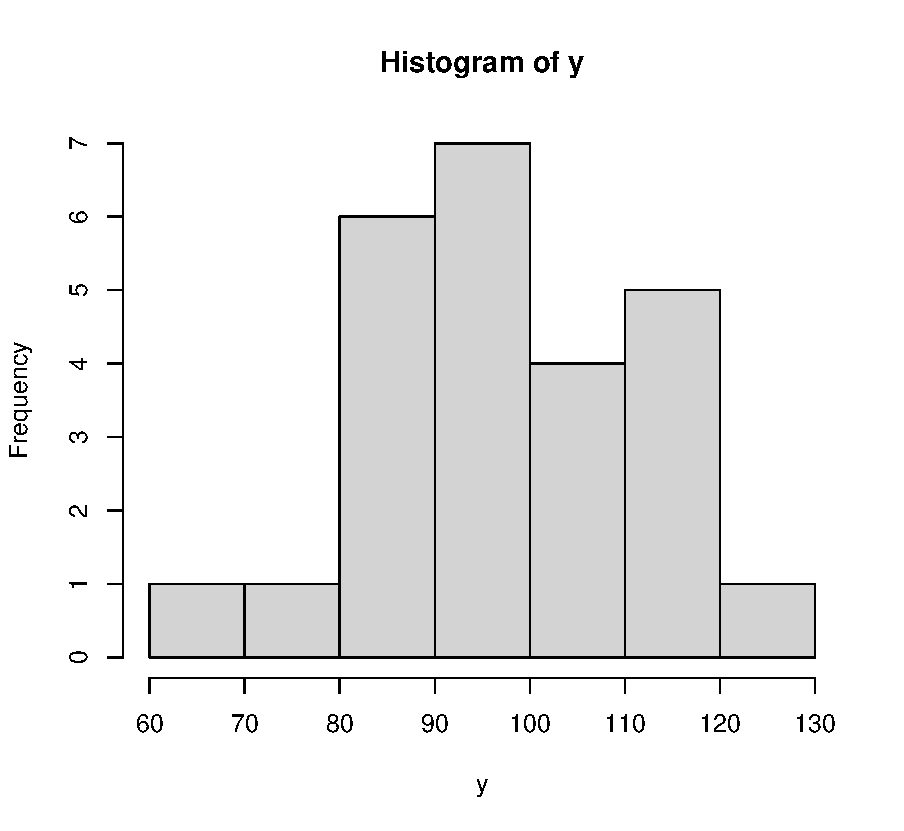
\includegraphics[width=.75\textwidth]{plot1.pdf}
		\end{figure}
		\lstinputlisting[language=R, firstline=51, lastline=52]{PS01_TB_23371290.R}
	\noindent I calculate the lower and upper bound for 90\% confidence level. \\  
	\lstinputlisting[language=R, firstline=64, lastline=66]{PS01_TB_23371290.R}
	\noindent Based on a 90\% confidence interval calculation for y, the CI ranges from 94.13283 to 102.7472 and the mean is 98.44. \\ 
	
	\item Next, the school counselor was curious  whether  the average student IQ in her school is higher than the average IQ score (100) among all the schools in the country.\\ 
	\noindent Using the same sample, conduct the appropriate hypothesis test with $\alpha=0.05$. \\


	\noindent Our hypothesis is average student IG is higher than the one in the country (100) and our null hypothesis is it is lower. P is lower or equals to 0.05. I already have mean (meany) and standard deviation (sde) as vectors. Before the p score, I need to find the z score. \\


	\lstinputlisting[language=R, firstline=79, lastline=80]{PS01_TB_23371290.R}
	\noindent I have the zscore as -1.56. I calculate the p score: \\
	\lstinputlisting[language=R, firstline=84, lastline=85]{PS01_TB_23371290.R}
	\noindent Our null hypothesis is correct since p is 1.94062 and lower than 5. We reject our hypothesis and can say that the average student IQ in the counselor`s school is lower than the average IQ score (100) among all the schools in the country.\\

\newpage

	\section*{Question 2 (40 points): Political Economy}

\noindent Researchers are curious about what affects the amount of money communities spend on addressing homelessness. The following variables constitute our data set about social welfare expenditures in the USA. \\
\vspace{.5cm}


\begin{tabular}{r|l}
	\texttt{State} &\emph{50 states in US} \\
	\texttt{Y} & \emph{per capita expenditure on shelters/housing assistance in state}\\
	\texttt{X1} &\emph{per capita personal income in state} \\
	\texttt{X2} &  \emph{Number of residents per 100,000 that are "financially insecure" in state}\\
	\texttt{X3} &  \emph{Number of people per thousand residing in urban areas in state} \\
	\texttt{Region} &  \emph{1=Northeast, 2= North Central, 3= South, 4=West} \\
\end{tabular}

\vspace{.5cm}
\noindent Explore the \texttt{expenditure} data set and import data into \texttt{R}.
\vspace{.5cm}
\begin{itemize}

\item
Please plot the relationships among \emph{Y}, \emph{X1}, \emph{X2}, and \emph{X3}? What are the correlations among them (you just need to describe the graph and the relationships among them)?
\vspace{.5cm}

\noindent After reviewing the table and adding Y, X1, X2, X3 as vectors for convenience, I researched online to plot all 4 variables. I used the ggplot approach detailed in `https://smin95.github.io/dataviz/basics-of-ggplot2-and-correlation-plot.html` and added the relevant packages. I use a variation of the below code to plot the relationships.\\
\lstinputlisting[language=R, firstline=119, lastline=120]{PS01_TB_23371290.R} 
\vspace{.5cm}


	\begin{figure}[h]\centering
		\caption{\footnotesize Relationship between Y, X1 and X2}
		\label{fig:plot_2}
		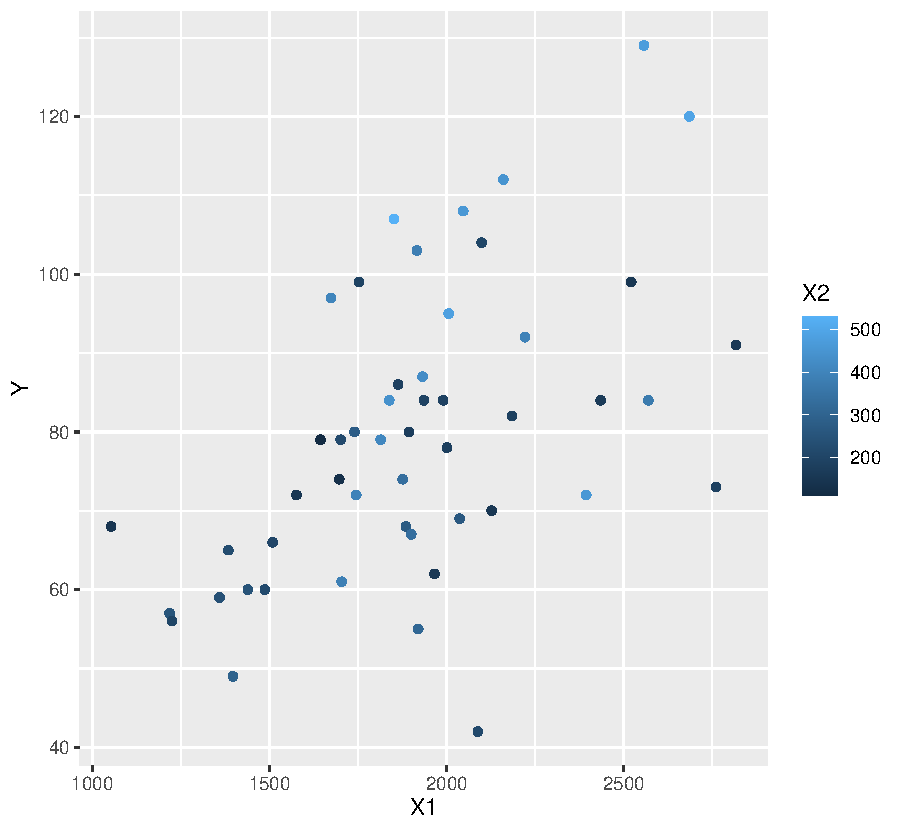
\includegraphics[width=.25\textwidth]{plot2.pdf}
	\end{figure}
	
	
\noindent Per Figure 2, there is positive correlation between Y and X1, but X2 is independent from both. It might be more meaningful to check the Y and X2. \\


				\begin{figure}[h]\centering
					\caption{\footnotesize Relationship between Y, X2 and X3}
					\label{fig:plot_3}
					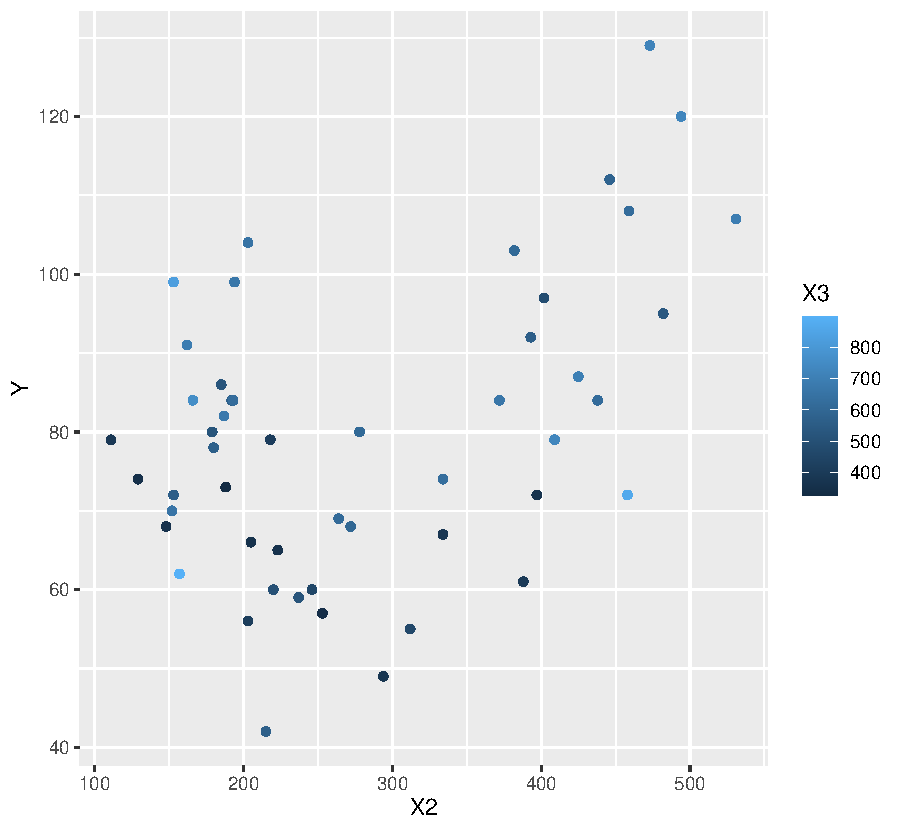
\includegraphics[width=.25\textwidth]{plot3.pdf}
				\end{figure}
				
				
	
\noindent Per Figure 3, there is no correlation between Y and X2, which is interesting. \\


				\begin{figure}[h]\centering
					\caption{\footnotesize Relationship between Y, X3 and X1}
					\label{fig:plot_4}
					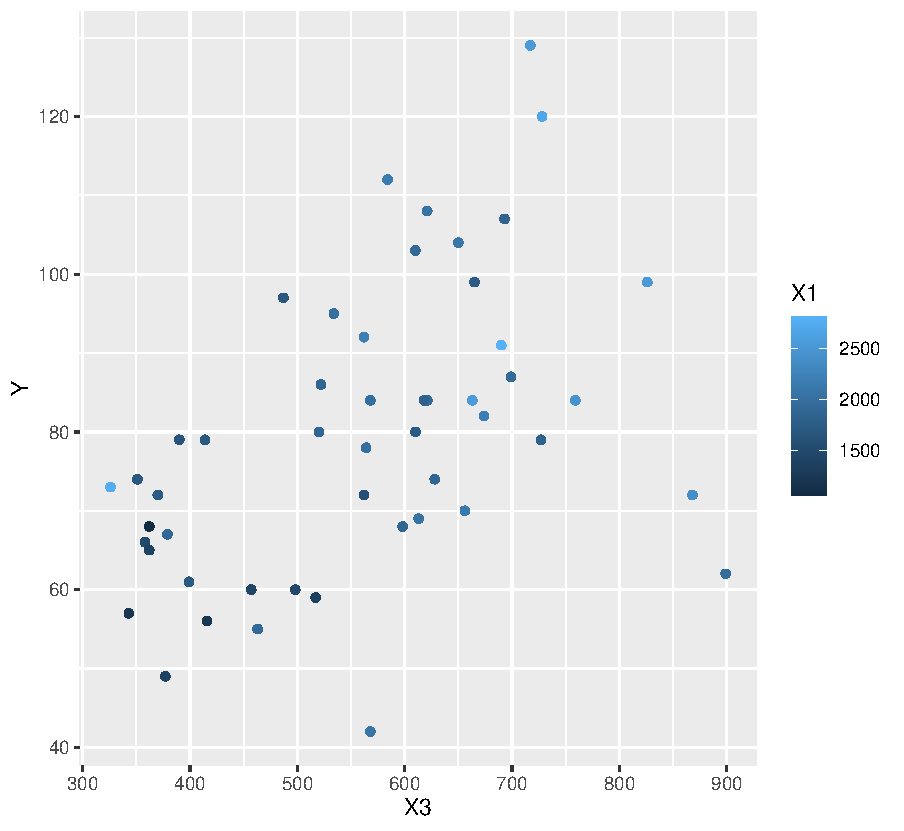
\includegraphics[width=.25\textwidth]{plot4.pdf}
				\end{figure}
				\vspace{.5cm}
	
\noindent Per Figure 4, there is a positive correlation between Y and X1. \\


\item
Please plot the relationship between \emph{Y} and \emph{Region}? On average, which region has the highest per capita expenditure on housing assistance?
	
	
	\noindent After some trial and error, and online research through these webpages, I created a ggplot. References: https://ggplot2.tidyverse.org/articles/faq-axes.html and https://stackoverflow.com/questions/39628480/plotting-median-of-the-points-in-r-ggplot \\
	\lstinputlisting[language=R, firstline=154, lastline=157]{PS01_TB_23371290.R} 
	\noindent Per Figure 5, region 4 has the highest per capita expenditure on housing assistance on average. On average, the highest per expenditure on housing assistance is ranked from highest: West, North Central, North East and South. \\
	
	
	\begin{figure}[h]\centering
	\caption{\footnotesize Relationship between Y, X3 and X2}
	\label{fig:plot_5}
	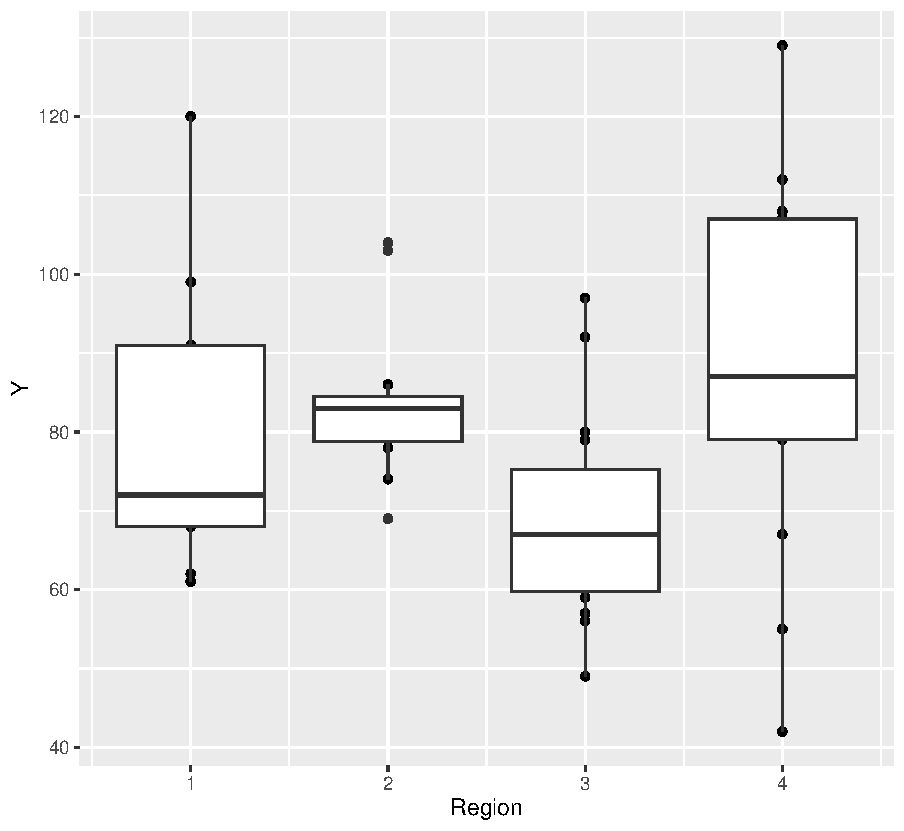
\includegraphics[width=.25\textwidth]{plot5.pdf}
	\end{figure}	




\item
Please plot the relationship between \emph{Y} and \emph{X1}? Describe this graph and the relationship. Reproduce the above graph including one more variable \emph{Region} and display different regions with different types of symbols and colors.


	\noindent On average, there is a positive correlation between per capita expenditure and per capita personal income in a state as seen on ggplot5. Again, I use https://smin95.github.io/dataviz/basics-of-ggplot2-and-correlation-plot.html as a reference to enrich my code and add the regions Figure 6. \\
	\lstinputlisting[language=R, firstline=180, lastline=182]{PS01_TB_23371290.R} 
		\begin{figure}[h]\centering
		\caption{\footnotesize Relationship between Y, and X1 with Regions}
		\label{fig:plot_6}
		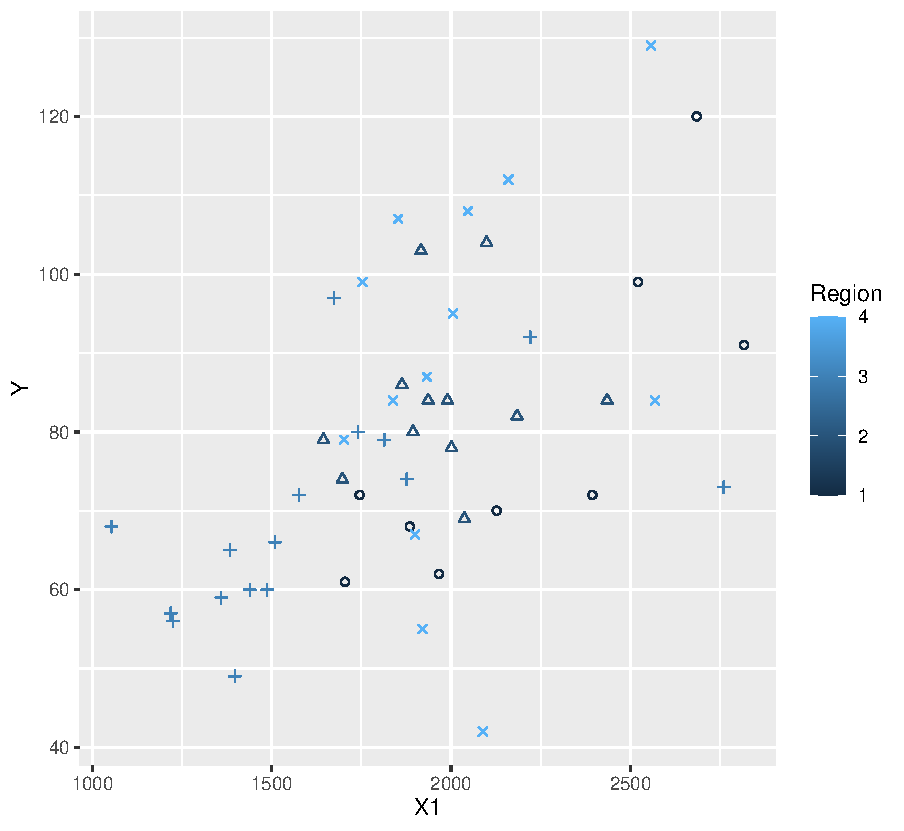
\includegraphics[width=.25\textwidth]{plot6.pdf}
		\end{figure}	
	\noindent I tried making the regions more readable on the shape but couldn't resolve the error. Nevertheless, o shape is Region 1, triangle is region 2, + is region 3 and x is Region 4 in Figure 6. \\
\end{itemize}

\end{document}